\documentclass{beamer}
%\documentclass[handout]{beamer}
%\documentclass[handout,notes=show]{beamer}

\usetheme{metropolis}

\usepackage{amsmath, amssymb, amsfonts, tikz}
\usepackage[utf8]{inputenc}
\usepackage[T1]{fontenc}
\usepackage[english]{babel}


\usepackage[default,scale=0.95]{opensans}

\usepackage{fontspec}
\usefonttheme{professionalfonts} % using non standard fonts for beamer
% \setsansfont[
% Path           = ~/.local/share/fonts/Google/TrueType/Open Sans/,
% Extension      = .ttf,
% Ligatures      = TeX,
% UprightFont    = OpenSans-Light,
% BoldFont       = OpenSans-Regular,
% ItalicFont     = OpenSans-LightItalic,
% BoldItalicFont = OpenSans-Italic
% ]{OpenSans}
% \setmonofont[
% Path           = ~/.local/share/fonts/Google/TrueType/Open Sans/,
% Extension      = .ttf,
% Ligatures      = TeX,
% UprightFont    = FiraCode-Regular,
% ItalicFont    = FiraCode-Regular,
% ItalicFont    = FiraCode-Regular,
% ]{DejaVu Sans Mono}
\metroset{block=fill}

% No navigation bars 
\beamertemplatenavigationsymbolsempty

\graphicspath{{img/}}

\definecolor{Purple}{HTML}{911146}
\definecolor{Orange}{HTML}{CF4A30}
\definecolor{Tan}{RGB}{225,221,191}
\definecolor{Green}{RGB}{76,131,122}
\definecolor{DB}{RGB}{4,37,58}

% Theme colors are derived from these two elements
\setbeamercolor{alerted text}{fg=Green}
\setbeamercolor{frametitle}{bg=Tan,fg=DB}
\usepackage{tabularx}
\usepackage{mathtools}
\usepackage{xmpmulti}
\usepackage{color}
\definecolor{keywordcolor}{rgb}{0.7, 0.1, 0.1}   % red
\definecolor{commentcolor}{rgb}{0.4, 0.4, 0.4}   % grey
\definecolor{symbolcolor}{rgb}{0.0, 0.1, 0.6}    % blue
\definecolor{sortcolor}{rgb}{0.1, 0.5, 0.1}      % green
\metroset{titleformat=smallcaps}


\newtheorem{proposition}[theorem]{Proposition}
\newtheorem{remarks}[theorem]{Remarks}
\newtheorem{remark}[theorem]{Remark}
\newtheorem{conjecture}[theorem]{Conjecture}


\theoremstyle{plain}
\newcommand{\terminology}[1]{\textbf{#1}}

\newcommand{\NN}{\mathbf{N}}
\newcommand{\ZZ}{\mathbf{Z}}
\newcommand{\QQ}{\mathbf Q}
\newcommand{\CC}{\mathbf C}
\newcommand{\RR}{\mathbf R}
\newcommand{\FF}{\mathbf F}
\newcommand{\lt}{<}
\newcommand{\gt}{>}
\newcommand{\amp}{&}
\newcommand{\diff}{\mathop{}\!\mathrm{d}}
\newcommand{\ints}{\mathcal{O}}
\newcommand{\ideal}[1]{\mathfrak{#1}}
\usepackage{mathrsfs}\usepackage{cancel}
\newcommand{\Gal}[2]{\operatorname{Gal}(#1/#2)}
\newcommand{\absgal}[1]{\operatorname{Gal}(\overline{#1}/#1)}
\DeclareMathOperator{\USp}{USp}
\DeclareMathOperator{\Spec}{Spec}

\newcommand{\sheaf}[1]{\operatorname{\mathcal{#1}}}
\newcommand{\inv}{^{-1}}
\DeclareMathOperator{\norm}{Nm}
\DeclareMathOperator{\ord}{ord}
\DeclareMathOperator{\divisor}{div}
\DeclareMathOperator{\PP}{\mathbf{P}}
\DeclareMathOperator{\Hom}{Hom}
\DeclareMathOperator{\Mat}{Mat}
\DeclareMathOperator{\End}{End}

\newcommand{\lb}{[}
\newcommand{\rb}{]}


\usepackage{listings}
\def\lstlanguagefiles{tex/lstlean.tex}

\lstset{language=lean,basicstyle=\ttfamily\scriptsize}

%\usepackage{mathfont}


\author{Alex J. Best}
\date{27/7/23 -- Rational points 2023 in Schney}
\title{Lean for the curious Arithmetic Geometer}

\begin{document}

\begin{frame}
  \titlepage

  \note[item]{Thank the audience for being awake.}
\end{frame}


\newcommand{\comment}[2]{#2}


\begin{frame}{Unit fractions}
    In December 2021 Thomas Bloom posted a paper: On a Density Conjecture about Unit Fractions to arXiv (2112.03726)
    \begin{quote}
        \textbf{Abstract:} We prove that any set $A \subset \mathbb{N}$ of positive upper density contains a finite $S \subset A$ such that $\sum_{n \in S} \frac{1}{n}=1$, answering a question of Erd\"os and Graham.
    \end{quote}
    18 pages, quickly recognized as correct and widely applauded in popular press (Quanta, etc), generalizes an older result of Croot. \pause

    Bloom and Mehta formalized the paper, over the following summer (2022).
    This took place before the referee report was complete, and the paper is still not published\pause

    (Bloom and Yael Dillies are right now working on formalizing Bloom-Sisask's variant (Feb 2023) on the Kelley-Meka bound on Roth numbers (also Feb 2023), bounding the size of subsets of the integers containing no three term arithmetic progressions)

    Upshot: at least in some areas of mathematics formalization is happening near concurrently with the work itself.
\end{frame}

\begin{frame}
    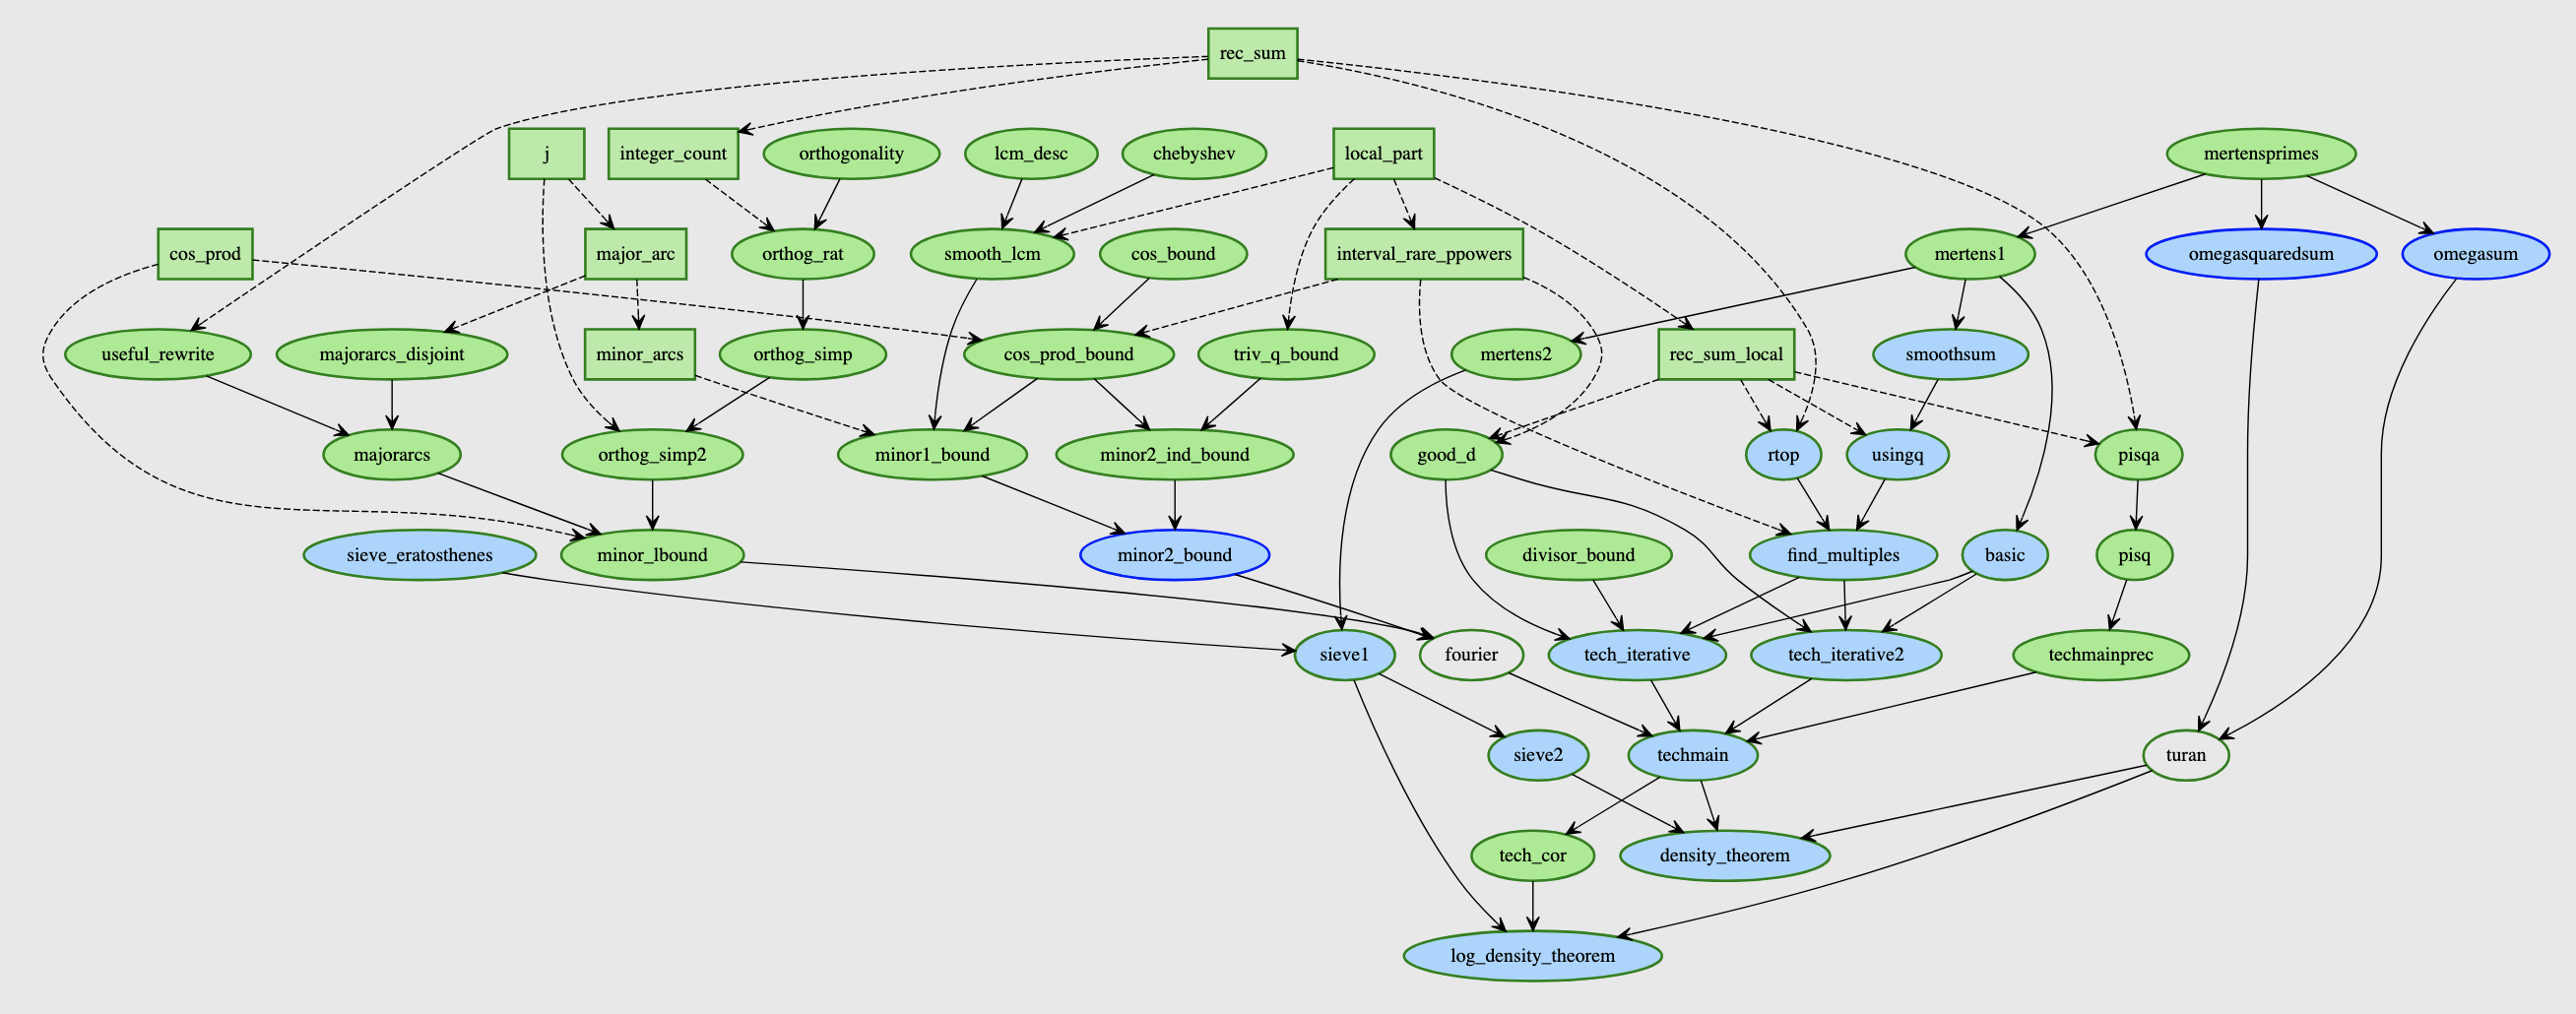
\includegraphics[width=1.1\linewidth]{unit.png}
\end{frame}

%\begin{frame}{Lindemann-Weierstrass}
%    In Coq and Isabelle
%\end{frame}
\begin{frame}{The Liquid Tensor Experiment}
    December 5, 2020, Peter Scholze
    \begin{quote}
        I want to propose a challenge: Formalize the proof of the following theorem:

        {\bf Theorem 1.1} (Clausen-S.): Let $0<p'<p\leq 1$ be real numbers, let $S$ be a profinite set, and let $V$ be a $p$-Banach space. Let $\mathcal M_{p'}(S)$ be the space of $p'$-measures on $S$. Then
        $\mathrm{Ext}^i_{\mathrm{Cond}(\mathrm{Ab})}(\mathcal M_{p'}(S),V)=0$
        for $i\geq 1$.

        Why do I want a formalization?
        ...

        —  ... I think the theorem is of utmost foundational importance, so being 99.9\% sure is not enough.
        ...
        — I spent much of 2019 obsessed with the proof of this theorem, almost getting crazy over it. In the end, we were able to get an argument pinned down on paper, but I think nobody else has dared to look at the details of this, and so I still have some small lingering doubts.
    \end{quote}
\end{frame}

\begin{frame}{The Liquid Tensor Experiment - Resolution}
    Around 20 people contributed in some way or another directly to the experiment. Though Johan Commelin and Adam Topaz were some of the most prolific, several others made serious contributions.

    In June 2021 the first "half" was completed, a technical analytical result, that was the heart of the difficulty of the proof.

    And one year later in July 2022 the cohomological part was completed, finishing the challenge after a year and a half.
\end{frame}

\begin{frame}{The Liquid Tensor Experiment - Resolution}
    In the course of the argument some of the mathematics was simplified, Commelin found a way to avoid the notion of Breen-Deligne resolutions, this was later found to be a reinvention of a complex introduced by Quillen.

    Many errors in the manuscript, some nontrivial were found and fixed during the process

    \begin{quote}
        Scholze:
        When I wrote the blog post half a year ago, I did not understand why the argument worked, and why we had to move from the reals to a certain ring of arithmetic Laurent series. But during the formalization, a significant amount of convex geometry had to be formalized, and this made me realize that actually the key thing happening is a reduction from a non-convex problem over the reals to a convex problem over the integers.
    \end{quote}
\end{frame}

\begin{frame}{The Liquid Tensor Experiment - Future}
    Many people are still interested in working with Condensed mathematics in a proof assistant.

    Dagur Asgeirsonn, a student of Clausen, is continuing to formalize new results from his thesis in a proof assistant.
\end{frame}

\begin{frame}{Rational points - Descent}
    With Baanen, Coppola, Dahmen, we have been formalizing some Mordell-style descent to find integral points on elliptic curves: for example the non-existence of integral points on
    $$y^2 = x^3 - 5$$

    This required computing the class group of $\QQ(\sqrt{-5})$ in a formally verified manner.
    (Baanen, Dahmen, Narayanan, Nuccio proved finiteness of the class group using a proof uniform in the number field and function field cases)

    It should be possible to go further, maybe even find rational points on appropriate higher genus curves.
    Generalizing a proof using a proof assistant is usually a lot of fun,
    copy paste the proof and see what breaks, sometimes very little does.
\end{frame}


\begin{frame}{What other sorts of things have been added to a proof assistant}
    \begin{itemize}
        \item Buzzard, Commelin, Massot: Perfectoid spaces
        \item Sophie Bernard: Lindemann-Weierstrass
        \item Avigad, Donnelly, Gray, Raff: Prime number theorem
        \item Michael Stoll: Legendre symbols, a nice proof of Quadratic Reciprocity, reciprocity for Hilbert symbols (in progress)
        \item Mar\'ia In\'es de Frutos-Fern\'andez: Adeles and ideles, defining Fontaines period rings, statement of main theorem of CFT
        \item Mar\'ia In\'es de Frutos-Fern\'andez and Filippo Nuccio: DVRs, general local fields, completions, with a view towards LCFT
            %\href{https://github.com/mariainesdff/local_class_field_theory}{(link)}
        \item Sophie Morel, formalization of half of her paper 
            ``Some combinatorial identities appearing in the calculation of the cohomology of Siegel modular varieties'' (with Ehrenborg and Readdy)
        \item Bernard, Cohen, Mahboubi, Strub + Browning: Abel--Ruffini theorem
    \end{itemize}
\end{frame}


\begin{frame}{Continued...}
    \begin{itemize}
        \item David Loeffler: Analytic continuation and functional equation of Riemann zeta, evaluation at negative integers
        \item Amelia Livingston: Group cohomology, Hilbert 90
        \item Lewis, Macbeth, Dupuis: Classify 1-d isocrystals
        \item Manuel Eberl, Chris Birkbeck: Modular forms
        \item Antoine Chambert-Loir and de Frutos-Fern\'andez: divided power structures
            \href{https://github.com/AntoineChambert-Loir/divided_powers}{(link)}
        \item David Angdinata and Junyan Xu: Group law on elliptic curves (in general), working on Mordell-Weil
        \item Brasca-B.-Birkbeck-Rodriguez: First case of FLT for regular primes.
        \item B.--Dahmen--Huriot-Tattegrain
        \item ... basics of schemes, Ostrowski's theorem...
        \item Your name here?: Your favourite moderately hard theorem
    \end{itemize}
\end{frame}

\begin{frame}{Lets Try!}
    First let's take a break.

    Afterwards we will do another short demo, we will help anyone interested get started with one of:

    Playing the Natural Number Game 4 (new and improved):
    \url{https://adam.math.hhu.de/\#/game/nng}

    Going through the Mathematics in Lean 4 tutorial:

    \url{https://github.com/leanprover-community/mathematics_in_lean}

    (you will need some form of computer for both, though both can be accessed via an online interface without installing anything)
\end{frame}

%\begin{frame}{Implementing number theoretic algorithms}
%\end{frame}

\begin{frame}{Implementing number theoretic algorithms}
    Alternatively we can implement algorithms within a proof assistant, as efficient functions that give the same output as what we want to compute
    \begin{itemize}
        \item Gives us a guaranteed correct implementation.
        \item We can experiment with modifying / improving the algorithm, and prove correctness or equality with the original one.
        \item We can prove properties, or "run" the algorithm in families, in ways normal code can't.
    \end{itemize}

    After writing the algorithm down, it is only accepted as a genuine mathematical function when it is shown to halt.
    With some functions this is obvious, but for algorithms that use recursion or unbounded loops, less so!
\end{frame}

\begin{frame}{Tate's algorithm}
    Sacha Huriot-Tattegrain (+B.+Dahmen) has implemented Tate's algorithm in Lean(4).

    \begin{itemize}
        \item Complete algorithm to compute local invariants of an elliptic curve, including the $c_p(E), \ord_p(\Delta_E), \ord_p(N_E)$

        \item Works in characteristic 2 and 3.

        \item Based on Cohen's description of the algorithm, but at times consulting other sources and even the GP source code was necessary to get it right.

        \item It runs fast!

        \item Partly generalized to base rings beyond $\ZZ$.
    \end{itemize}

    Without an independent definition of the Kodaira types and conductor exponent we cannot actually check the algorithm does what it says.
    Nevertheless we could prove certain properties of the algorithm in future, such as invariance under change of the initial model.
\end{frame}

\begin{frame}{Closing thoughts}
    Formalization of mathematics (including number theory) is still slow and painful at times.

    But we have several decades, even thousands of years of mathematics itself, learning how to think about mathematics, and to explain mathematics, to catch up on.

    Thinking about these issues and finding clean arguments can be a lot of fun, and the tool may occasionally surprise you.
\end{frame}


\comment{



\begin{frame}{Some examples: Grunwald(-Wang) and K-theory}

    \begin{quotation}
        Some days later I was with Artin in his office when Wang appeared. He said he had a counterexample to a lemma which had been used in the proof. An hour or two later, he produced a counterexample to the theorem itself... Of course he [Artin] was astonished, as were all of us students, that a famous theorem with two published proofs, one of which we had all heard in the seminar without our noticing anything, could be wrong.

        --- Tate
    \end{quotation}\pause

    \note{The problem: 2, the cursed prime. This is often an edge case.}

    \begin{quotation}
        The groundbreaking 1986 paper “Algebraic Cycles and Higher K-theory” by Spencer Bloch was soon after publication found by Andrei Suslin to contain a mistake in the proof of Lemma 1.1. The proof could not be fixed.

        --- Voevodsky
    \end{quotation}

\end{frame}

\begin{frame}{The solution: Take 2}
    What if computers could do the boring work for us?\pause

    Computers are:
    \begin{itemize}
        \item Capable of checking basic logical statements,\pause
        \item Fast,\pause
        \item Never complain.
    \end{itemize}
\end{frame}

\begin{frame}{The new problem}
    How do you describe the steps of a proof to a computer with as little pain as possible? \pause
    Often mathematicians leave unsaid many steps which are intuitive or easily supplied. \note{(this is one place mistakes enter)}\pause

    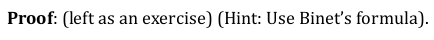
\includegraphics[height=2em]{pf-exercise.png}\pause

    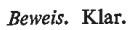
\includegraphics[height=1.5em]{beweis-klar.png}\pause

    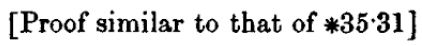
\includegraphics[height=1.5em]{pf-similar.png}\pause

    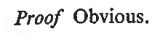
\includegraphics[height=2em]{pf-obvious.png}\pause

    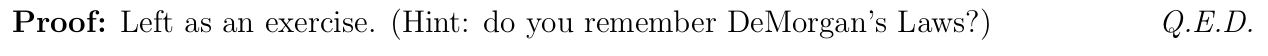
\includegraphics[height=1.5em]{pf-remember.png}\pause

    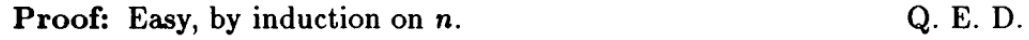
\includegraphics[height=1.1em]{pf-easy-induct.png}\pause

    The computer will probably not understand these, but in order to stay sane we must strike a balance between detail and verbosity.\note{ Teach the computer to work off as little as possible.}
\end{frame}

\begin{frame}{Enter Lean}
    The idea of trying this sort of thing has been around for a while. \pause

    But only within the last few years has it begun to seem more feasible for an average mathematician to do this. Tools have gotten better, slowly this idea has gained traction.\pause

    Recently an interactive proof assistant called Lean has been under heavy development. And I've been playing with it.

    Let me show you some lean code:
\end{frame}

\begin{frame}[fragile]
\begin{lstlisting}
lemma fact_rec (n : ℕ) :
factorial (n + 1) = factorial n * (n+1) :=
begin
-- write out the definition of factorial
unfold factorial,
-- remember {1,...,n+1} = {1,...,n} ∪ {n+1}
rewrite list.range'_concat 1 n,
-- the product of two sequences joined together is just the product of the products of each sequence
rewrite list.prod_append,
-- I'm bored already are we done here?
simp,
-- YES!
end
\end{lstlisting}\pause
We can replace all of the above with: \lstinline{by unfold factorial; simp [list.range'_concat, list.prod_append]}
\note{ Lean will figure out when and how to apply the lemmas.}

\end{frame}

\begin{frame}{(not so?) Live demo!}
    \multiinclude[<+->][format=png, graphics={width=\textwidth}]{fact}
\end{frame}

\begin{frame}{But can it do research?}
    But the basics of algebraic number theory are not really complete (Kummer-Dedekind, Kummer theory, Kronecker-Weber) in any formal system that I know.
    Research level mathematics requires a vast body of knowledge to even think about.
    \pause

    As humans we forget this and also gloss over things we (think we) know well.
    \pause

    For instance one can forget what a Dedekind cut is, or Peano arithmetic and still think about real and natural numbers without an issue.
    Our intuition allows us to abstract these concepts so far away that we don't have to work from the ground up when approaching a problem.

\end{frame}}

\end{document}
